% !Mode:: "TeX:UTF-8"
% 1. Install CTeX; 2. Update WinEdt; 3. Update MiKTeX
% ses: http://www.ctex.org/OnlineDocuments, https://www.overleaf.com/learn
% add package,  texhash
% error: miktex-makemf: The umvs source file could not be found. solution: initexmf --mkmaps & initexmf --update-fndb


\documentclass[12pt,UTF8]{ctexart}%{jmlr}%{ctexart}%{article}%

\usepackage{longtable}
\usepackage{booktabs}
\usepackage{syntonly}
\usepackage{ulem}
%\usepackage{amsmath}
\usepackage{mathtools}
\usepackage{amssymb}
\usepackage{amsthm}
\usepackage{xcolor}
\usepackage{hyperref}
\hypersetup{hidelinks} % or: \hypersetup{pdfborder={0 0 0}}

\usepackage{tikz}
%\usepackage{latexsym}
%\syntaxonly
%\usepackage[utf8]{inputenc}

%\usepackage(pei)



\title{Chapter 1. The introduction of \LaTeX}

\begin{document}


\section{模板}

https://www.overleaf.com/latex/templates/

https://www.latexstudio.net/

http://www.latextemplates.com/

https://github.com/DeathKing/LaTeX-Template-Cn


\section{Test}
Hello this is a document content

中文测试

\begin{center}
满纸荒唐言\\
一把辛酸泪\\
都云作者痴\\
谁解其中味\\
\end{center}

\newpage
\section{排版}
1.
Several spaces equal one.
Front spaces are ignored.
An empty line starts a new
paragraph.\par
A \verb|\par| command also
starts a new line.

2.
\# \$ \% \& \{ \} \_
\^{} \~{} \textbackslash

3.连字\par
It's difficult to find \ldots .\par
It's dif{}f{}icult to f{}ind \ldots .

4.标点\par
``Please press the `x' key."\par
daughter-in-law, X-rated\par
pages 13--67\par
yes---or no?\par
one, two, three, \dots one hundred\par

5.西文\par
H\^otel, na\"\i ve, \'el\`eve,\par
sm\o rrebr\o d, !`Se\ norita!,\par
Sch\"onbrunner Schlo\ss{}\par
Stra\ss e

6.其他符号\par
\P{} \S{} \dag{} \ddag{}\
\copyright{} \pounds{}\
\textasteriskcentered\
\textperiodcentered\
\textbullet\
\textregistered{} \texttrademark


\newpage

7.强调\par
An \underline{underlined} text.\par
An example of \uline{some long and underlined words.}\par

Some \emph{emphasized words,
including \emph{double-emphasized}
words}, are shown here.


8.单词间距和断行\par
Fig.~2a. \~{}不断行空格\\
Donale~E. Knuth

9.手动断词\par
You can find some long text break new line. I think this is: su\-per\-cal\-%
i\-frag\-i\-lis\-tic\-ex\-pi\-%
al\-i\-do\-cious.


\newpage
\section{文档元素}

1. 标题\par
\textbackslash chapter\{title\} \textbackslash section\{title\} \textbackslash subsection\{title\}
\textbackslash subsubsection\{title\} \textbackslash paragraph\{title\} \textbackslash subparagraph\{title\}


2.引用\par
A reference to this subsection
\label{sec:this} looks like:
``see section~\ref{sec:this} on
page~\pageref{sec:this}.''

3.脚注\par
“天地玄黄,宇宙洪荒。日月盈昃,辰宿列张。”\footnote{出自《千字文》。}\par
\par
\begin{tabular}{l}
\hline
“天地玄黄,宇宙洪荒。日月盈昃,辰宿列张。”\footnotemark \\
\hline
\end{tabular}
\footnotetext{表格里的名句出自《千字文》。} \par

\marginpar{\footnotesize 边注较窄,不要写过多文字,最好设置较小的字号。}

4.列表\par
\begin{enumerate}
\item An item.
\begin{enumerate}
\item A nested item.\label{itref}
\item[*] A starred item.
\end{enumerate}
\item Reference(\ref{itref}).
\end{enumerate}\par


\begin{itemize}
\item An item.
\begin{itemize}
\item A nested item.
\item[+] A `plus' item.
\item Another item.
\end{itemize}
\item Go back to upper level.
\end{itemize}



\begin{description}
\item[Enumerate] Numbered list.
\item[Itemize] Non-numbered list.
\end{description}




\renewcommand{\labelitemi}{\ddag}
\renewcommand{\labelitemii}{\dag}
\begin{itemize}
\item First item
\begin{itemize}
\item Subitem
\item Subitem
\end{itemize}
\item Second item
\end{itemize}



\renewcommand{\labelenumi}%
{\Alph{enumi}}
\begin{enumerate}
\item First item
\item Second item
\end{enumerate}


\newpage
5. 对齐环境\par

\begin{center}
Centered text using a
\verb|center| environment.
\end{center}
\begin{flushleft}
Left-aligned text using a
\verb|flushleft| environment.
\end{flushleft}
\begin{flushright}
Right-aligned text using a
\verb|flushright| environment.
\end{flushright}



6.引用环境\par

Francis Bacon says:
\begin{quote}
Knowledge is power.
\end{quote}


《木兰诗》:
\begin{quotation}
万里赴戎机,关山度若飞。
朔气传金柝,寒光照铁衣。
将军百战死,壮士十年归。
归来见天子,天子坐明堂。
策勋十二转,赏赐百千强。……
\end{quotation}


Rabindranath Tagore's short poem:
\begin{verse}
Beauty is truth's smile
when she beholds her own face in
a perfect mirror.
\end{verse}

7. 代码环境\par

\begin{verbatim}
#include <iostream>
int main()
{
std::cout << "Hello, world!"
<< std::endl;
return 0;
}
\end{verbatim}

\begin{verbatim*}
for (int i=0; i<4; ++i)
printf("Number %d\n",i);
\end{verbatim*}


\verb|\LaTeX| \\
\verb+(a || b)+ \verb*+(a || b)+


8.表格\par

\begin{tabular}{|c|}
center-\\ aligned \\
\end{tabular},
\begin{tabular}[t]{|c|}
top-\\ aligned \\
\end{tabular},
\begin{tabular}[b]{|c|}
bottom-\\ aligned\\
\end{tabular} tabulars.\par

\par

\begin{tabular}{lcr|p{6em}}
\hline
left & center & right
& par box with fixed width\\
L & C & R & P \\
\hline
\end{tabular}\par


\begin{tabular}{@{} r@{:}lr @{}}
\hline
1 & 1 & one \\
11 & 3 & eleven \\
\hline
\end{tabular}

9.图片\par
%\includegraphics{assets/th.jpg}
\includegraphics[scale=0.7,angle=90]{assets/th.jpg}


10.盒子\par

|\mbox{Test some words.}|\\
|\makebox[10em]{Test some words.}|\\
|\makebox[10em][l]{Test some words.}|\\
|\makebox[10em][r]{Test some words.}|\\
|\makebox[10em][s]{Test some words.}|


\fbox{Test some words.}\\
\framebox[10em][r]{Test some words.}


\framebox[10em][r]{Test box}\\[1ex]
\setlength{\fboxrule}{1.6pt}
\setlength{\fboxsep}{1em}
\framebox[10em][r]{Test box}

垂直盒子:
\par
三字经:\parbox[t]{3em}%
{人之初 性本善 性相近 习相远}
\quad
千字文:
\begin{minipage}[b][8ex][t]{4em}
天地玄黄 宇宙洪荒
\end{minipage}


\fbox{\begin{minipage}{15em}%
这是一个垂直盒子的测试。
\footnote{脚注来自 minipage。}
\end{minipage}}

标尺:
\par
Black \rule{12pt}{4pt} box.
Upper \rule[4pt]{6pt}{8pt} and
lower \rule[-4pt]{6pt}{8pt} box.
A \rule[-.4pt]{3em}{.4pt} line.


11.浮动体\par



\section{排版数学公式}

1.行内和行间公式

The Pythagorean theorem is
$a^2 + b^2 = c^2$.


The Pythagorean theorem is:
\begin{equation}
a^2 + b^2 = c^2 \label{pythagorean}
\end{equation}
Equation \eqref{pythagorean} is
called `Gougu theorem' in Chinese.



It's wrong to say
\begin{equation}
1 + 1 = 3 \tag{dumb}
\end{equation}
or
\begin{equation}
1 + 1 = 4 \notag
\end{equation}


\begin{equation*}
a^2 + b^2 = c^2
\end{equation*}
For short:
\[ a^2 + b^2 = c^2 \]
Or if you like the long one:
\begin{displaymath}
a^2 + b^2 = c^2
\end{displaymath}


In text:
$\lim_{n \to \infty}
\sum_{k=1}^n \frac{1}{k^2}
= \frac{\pi^2}{6}$.
In display:
\[
\lim_{n \to \infty}
\sum_{k=1}^n \frac{1}{k^2}
= \frac{\pi^2}{6}
\]


$x^{2} \geq 0 \qquad
\text{for \textbf{all} }
x\in\mathbb{R}$


\subsection{数学符号}

\subsubsection{一般符号}

$\alpha$ $\beta$ $\Gamma$ $\Delta$
$\epsilon$ $\varepsilon$ $\zeta$ $\eta$ $\theta$ $\vartheta$ $\Theta$
$\iota$ $\kappa$ $\lambda$ $\mu$
$\xi$ $\pi$ $\rho$ $\varrho$
$\sigma$ $\tau$ $\upsilon$ $\phi$ $\varphi$
$\chi$ $\psi$


$a_1, a_2, \dots, a_n$ \\
$a_1 + a_2 + \cdots + a_n$ \par

\subsubsection{指数、上下标和导数}

$p^3_{ij} \qquad
m_\mathrm{Knuth}\qquad
\sum_{k=1}^3 k $\\[5pt]
$a^x+y \neq a^{x+y}\qquad
e^{x^2} \neq {e^x}^2$\par

$f(x) = x^2 \quad f'(x)
= 2x \quad f''^{2}(x) = 4$

\subsubsection{分式和根式}

1. 分式\par

In display style:
\[
3/8 \qquad \frac{3}{8}
\qquad \tfrac{3}{8}
\]

In text style:
$1\frac{1}{2}$~hours \qquad
$1\dfrac{1}{2}$~hours

2.根式\par

$\sqrt{x} \Leftrightarrow x^{1/2}
\quad \sqrt[3]{2}
\quad \sqrt{x^{2} + \sqrt{y}}$

3.特殊\par
Pascal's rule is
\[
\binom{n}{k} =\binom{n-1}{k}
+ \binom{n-1}{k-1}
\]


\subsubsection{关系符}

$\neq\doteq\propto<>$

\[
f_n(x) \stackrel{*}{\approx} 1
\]

\subsubsection{算符}
$\times \div \cdot \pm \mp \nabla \partial$

\[
\lim_{x \rightarrow 0}
\frac{\sin x}{x}=1
\]

$a\bmod b, x\equiv a \pmod{b}$

\subsubsection{巨算符}

In text:
$\sum_{i=1}^n \quad
\int_0^{\frac{\pi}{2}} \quad
\oint_0^{\frac{\pi}{2}} \quad
\prod_\epsilon $ \\
In display:
\[\sum_{i=1}^n \quad
\int_0^{\frac{\pi}{2}} \quad
\oint_0^{\frac{\pi}{2}} \quad
\prod_\epsilon \]



In text:
$\sum\limits_{i=1}^n \quad
\int\limits_0^{\frac{\pi}{2}} \quad
\prod\limits_\epsilon $ \\
In display:
\[\sum\nolimits_{i=1}^n \quad
\int\limits_0^{\frac{\pi}{2}} \quad
\prod\nolimits_\epsilon \]


\[
\sum_{\substack{0\le i\le n \\
j\in \mathbb{R}}}
P(i,j) = Q(n)
\]
\[
\sum_{\begin{subarray}{l}
0\le i\le n \\
j\in \mathbb{R}
\end{subarray}}
P(i,j) = Q(n)
\]


\subsubsection{数学重音和上下括号}

$\bar{x_0} \quad \bar{x}_0$\\[5pt]
$\vec{x_0} \quad \vec{x}_0$\\[5pt]
$\hat{\mathbf{e}_x} \quad
\hat{\mathbf{e}}_x$


$0.\overline{3} =
\underline{\underline{1/3}}$ \\[5pt]
$\hat{XY} \qquad \widehat{XY}$\\[5pt]
$\vec{AB} \qquad
\overrightarrow{AB}$

$\underbrace{\overbrace{(a+b+c)}^6
\cdot \overbrace{(d+e+f)}^7}
_\text{meaning of life} = 42$


\subsubsection{箭头}

\[ a\xleftarrow{x+y+z} b \]
\[ c\xrightarrow[x<y]{a*b*c}d \]


\subsubsection{括号和定界符}

${a,b,c} \neq \{a,b,c\}$

\[1 + \left(\frac{1}{1-x^{2}}
\right)^3 \qquad
\left.\frac{\partial f}{\partial t}
\right|_{t=0}\]


$\Bigl((x+1)(x-1)\Bigr)^{2}$\\
$\bigl( \Bigl( \biggl( \Biggl( \quad
\bigr\} \Bigr\} \biggr\} \Biggr\} \quad
\big\| \Big\| \bigg\| \Bigg\| \quad
\big\Downarrow \Big\Downarrow
\bigg\Downarrow \Bigg\Downarrow$


\subsection{多行公式}

\subsubsection{长公式折行}

\begin{multline}
a + b + c + d + e + f
+ g + h + i \\
= j + k + l + m + n\\
= o + p + q + r + s\\
= t + u + v + x + z
\end{multline}


\subsubsection{多行公式}

\begin{align}
a & = b + c \\
& = d + e
\end{align}


\begin{align}
a ={} & b + c \\
={} & d + e + f + g + h + i
+ j + k + l \notag \\
& + m + n + o \\
={} & p + q + r + s
\end{align}

\begin{align}
a &=1 & b &=2 & c &=3 \\
d &=-1 & e &=-2 & f &=-5
\end{align}

\begin{gather}
a = b + c \\
d = e + f + g \\
h + i = j + k \notag \\
l + m = n
\end{gather}


\subsubsection{公用编号的多行公式}

\begin{equation}
\begin{aligned}
a &= b + c \\
d &= e + f + g \\
h + i &= j + k \\
l + m &= n
\end{aligned}
\end{equation}


\subsection{数组和矩阵}

\[ \mathbf{X} = \left(
\begin{array}{cccc}
x_{11} & x_{12} & \ldots & x_{1n}\\
x_{21} & x_{22} & \ldots & x_{2n}\\
\vdots & \vdots & \ddots & \vdots\\
x_{n1} & x_{n2} & \ldots & x_{nn}\\
\end{array} \right) \]

\[ |x| = \left\{
\begin{array}{rl}
-x & \text{if } x < 0,\\
0 & \text{if } x = 0,\\
x & \text{if } x > 0.
\end{array} \right. \]

\[ |x| =
\begin{cases}
-x & \text{if } x < 0,\\
0 & \text{if } x = 0,\\
x & \text{if } x > 0.
\end{cases} \]

\[
\begin{matrix}
1 & 2 \\ 3 & 4
\end{matrix} \qquad
\begin{bmatrix}
x_{11} & x_{12} & \ldots & x_{1n}\\
x_{21} & x_{22} & \ldots & x_{2n}\\
\vdots & \vdots & \ddots & \vdots\\
x_{n1} & x_{n2} & \ldots & x_{nn}\\
\end{bmatrix}
\]


\[
\mathbf{H}=
\begin{bmatrix}
\dfrac{\partial^2 f}{\partial x^2} &
\dfrac{\partial^2 f}
{\partial x \partial y} \\[8pt]
\dfrac{\partial^2 f}
{\partial x \partial y} &
\dfrac{\partial^2 f}{\partial y^2}
\end{bmatrix}
\]



\subsection{公式中的间距}

\[
\int_a^b f(x)\mathrm{d}x
\qquad
\int_a^b f(x)\,\mathrm{d}x
\]

\newcommand\diff{\,\mathrm{d}}
\begin{gather*}
\int\int f(x)g(y)
\diff x \diff y \\
\int\!\!\!\int
f(x)g(y) \diff x \diff y \\
\iint f(x)g(y) \diff x \diff y \\
\iint\quad \iiint\quad \idotsint
\end{gather*}


\subsection{数学符号的字体控制}

\subsubsection{数学字母字体}

$\mathcal{R} \quad \mathfrak{R}
\quad \mathbb{R}$
\[\mathcal{L}
= -\frac{1}{4}F_{\mu\nu}F^{\mu\nu}\]
$\mathfrak{su}(2)$ and
$\mathfrak{so}(3)$ Lie algebra

\subsubsection{数学符号的尺寸}

\[
P = \frac
{\sum_{i=1}^n (x_i- x)(y_i- y)}
{\displaystyle \left[
\sum_{i=1}^n (x_i-x)^2
\sum_{i=1}^n (y_i-y)^2
\right]^{1/2} }
\]


\subsubsection{加粗的数学符号}

$\mu, M \qquad
\mathbf{\mu}, \mathbf{M}$
\qquad {\boldmath$\mu, M$}


\subsection{定理环境}

\subsubsection{原始的定理环境}

\newtheorem{mythm}{My Theorem}[section]
\begin{mythm}\label{thm:light}
The light speed in vacuum
is $299,792,458\,\mathrm{m/s}$.
\end{mythm}

\begin{mythm}[Energy-momentum relation]
The relationship of energy,
momentum and mass is
\[E^2 = m_0^2 c^4 + p^2 c^2\]
where $c$ is the light speed
described in theorem \ref{thm:light}.
\end{mythm}

\subsubsection{amsthm 宏包}


\subsubsection{证明环境和证毕符号}

\begin{proof}
For simplicity, we use
\[
E=mc^2
\]
That's it.
\end{proof}

\begin{proof}
For simplicity, we use
\[
E=mc^2 \qedhere
\]
\end{proof}

\begin{proof}
Assuming $\gamma
= 1/\sqrt{1-v^2/c^2}$, then
\begin{align*}
E &= \gamma m_0 c^2 \\
p &= \gamma m_0v \qedhere
\end{align*}
\end{proof}

\begin{proof}
For simplicity, we use
\begin{equation}
E=mc^2.\qedhere
\end{equation}
\end{proof}

\renewcommand{\qedsymbol}%
{\rule{1ex}{1.5ex}}
\begin{proof}
For simplicity, we use
\[
E=mc^2 \qedhere
\]
\end{proof}

\subsection{符号表}


\section{排版样式设定}

\subsection{字体和字号}

{\small The small and
\textbf{bold} Romans ruled}
{\Large all of great big
{\itshape Italy}.}

\subsubsection{字体样式}

\subsubsection{字号}

He likes {\LARGE large and
{\small small} letters}.

\subsection{段落格式和间距}

\subsubsection{行距}

{\linespread{2.0}\selectfont
The baseline skip is set to be
twice the normal baseline skip.
Pay attention to the \verb|\par|
command at the end. \par}
In comparison, after the
curly brace has been closed,
everything is back to normal.

{\Large Don't read this!
It is not true.
You can believe me!\par}

{\Large This is not true either.
But remember I am a liar.}\par


\subsubsection{段落格式}

\setlength{\parskip}{1ex plus 0.5ex minus 0.2ex}

In comparison, after the
curly brace has been closed,
everything is back to normal.


\subsubsection{水平间距}

This\hspace{1.5cm}is a space
of 1.5 cm.

x\hspace{\stretch{1}}
x\hspace{\stretch{3}}
x\hspace{\fill}x

{\Large big\hspace{1em}y}\\
{\Large big\quad y}\\
nor\hspace{2em}mal\\
nor\qquad mal\\
{\tiny tin\hspace{1em}y}\\
{\tiny tin\quad y}


\subsubsection{垂直间距}

A paragraph.\par
\vspace{2ex}
Another paragraph.

Use command \verb|\vspace{12pt}|
to add \vspace{12pt} some spaces
between lines in a paragraph.
Or you can use \verb|\\[12pt]|
to \\[12pt] add vertical space,
but it also breaks the paragraph.

\parbox[t]{3em}{TeX\par TeX}
\parbox[t]{3em}{TeX\par\smallskip TeX}
\parbox[t]{3em}{TeX\par\medskip TeX}
\parbox[t]{3em}{TeX\par\bigskip TeX}

\subsection{页面和分栏}

\subsubsection{利用 geometry 宏包设置页面参数}

\subsection{页眉页脚}


\section{特色工具和功能}

\subsection{参考文献和 BIBTEX 工具}

\subsection{索引和 makeindex 工具}

\subsection{使用颜色}

\subsubsection{颜色的表达方式(color,xcolor)}

\large\sffamily
{\color[gray]{0.6}
60\% 灰色} \\
{\color[rgb]{0,1,1}
青色}

\large\sffamily
{\color{red} 红色} \\
{\color{blue} 蓝色}

\large\sffamily
{\color{red!40} 40\% 红色}\\
{\color{blue}蓝色
\color{blue!50!black}蓝黑
\color{black}黑色}\\
{\color{-red}红色的互补色}

\subsubsection{带颜色的文本和盒子}

\sffamily
文字用\textcolor{red}{红色}强调\\
\colorbox[gray]{0.95}{浅灰色背景} \\
\fcolorbox{blue}{yellow}{%
\textcolor{blue}{蓝色边框+文字,%
黄色背景}
}


\subsection{使用超链接}


\subsubsection{hyperref}

\url{http://wikipedia.org} \\
\href{http://wikipedia.org}{Wiki}


\subsubsection{PDF 书签}

质能公式 \texorpdfstring{$E=mc^2$}{E=mc\textasciicircum 2}


\section{绘图功能}

\subsection{ TikZ 绘图语言}


\subsubsection{TikZ 坐标和路径}

1.\par
\begin{tikzpicture}
\draw (0,0) -- (30:1);
\draw (1,0) -- (2,1);
\coordinate (S) at (0,1);
\draw (S) -- (1,1);
\end{tikzpicture}

2.\par
\begin{tikzpicture}
\coordinate (S) at (2,2);
\draw[gray] (-1,2) -- (S);
\draw[gray] (2,-1) -- (S);
\draw[red] (0,0) -- (0,0 -| S);
\draw[blue] (0,0) -- (0,0 |- S);
\end{tikzpicture}

3.\par
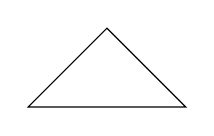
\begin{tikzpicture}
\draw (0,0) -- (1,1) -- (2,0) -- cycle;
\end{tikzpicture}

4.\par
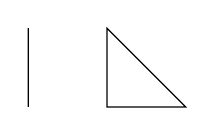
\begin{tikzpicture}
\draw (0,0) -- (0,1)
(1,0) -- (1,1) -- (2,0) -- cycle;
\end{tikzpicture}

5.\par
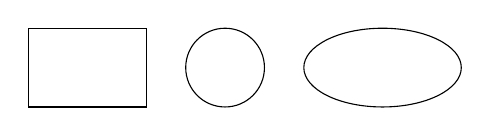
\begin{tikzpicture}
\draw (0,0) rectangle (1.5,1);
\draw (2.5,0.5) circle [radius=0.5];
\draw (4.5,0.5) ellipse
[x radius=1,y radius=0.5];
\end{tikzpicture}

6.\par
\begin{tikzpicture}
\draw (0,0) |- (1,1);
\draw (1,0) -| (2,1);
\draw (4,0) arc (0:135:1);
\draw (6,0) arc (0:135:1 and 0.5);
\end{tikzpicture}

7.\par

\begin{tikzpicture}
\draw (0,0) sin (1,1);
\draw (0,1) sin (1,0);
\draw (2,1) cos (3,0);
\draw (2,0) cos (3,1);
\end{tikzpicture}

8.\par
\begin{tikzpicture}
\draw (0,0) parabola (1,2);
\draw (2,0) parabola
bend (2.25,-0.25) (3,2);
\draw (4,0) parabola
bend (4.75,2.25) (5,2);
\end{tikzpicture}

9.\par
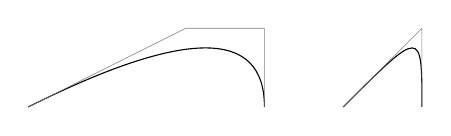
\begin{tikzpicture}
\draw (0,0) .. controls
(2,1) and (3,1) .. (3,0);
\draw (4,0) .. controls
(5,1) .. (5,0);
\draw[help lines] (0,0)
-- (2,1) -- (3,1) -- (3,0)
(4,0) -- (5,1) -- (5,0);
\end{tikzpicture}

10.\par
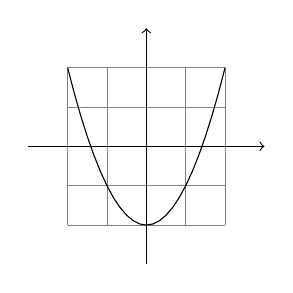
\begin{tikzpicture}
\draw[help lines,step=0.5]
(-1,-1) grid (1,1);
\draw[->] (-1.5,0) -- (1.5,0);
\draw[->] (0,-1.5) -- (0,1.5);
\draw[domain=-1:1]
plot(\x,{\x*\x*2 -1});
\end{tikzpicture}

\subsubsection{ TikZ 绘图命令和参数}

1.\par

\begin{tikzpicture}[thick]
\draw[blue] (0,0) rectangle (1,1);
\filldraw[fill=yellow,draw=red]
(2,0.5) circle [radius=0.5];
\end{tikzpicture}

2.\par

\begin{tikzpicture}
\draw[ultra thin] (0,0)--(0,2);
\draw[very thin] (0.5,0)--(0.5,2);
\draw[thin] (1,0)--(1,2);
\draw[semithick] (1.5,0)--(1.5,2);
\draw[thick] (2,0)--(2,2);
\draw[very thick] (2.5,0)--(2.5,2);
\draw[ultra thick] (3,0)--(3,2);
\end{tikzpicture}

3.\par
\begin{tikzpicture}
\draw[dashed] (0,0) -- (0,2);
\draw[dotted] (0.5,0) -- (0.5,2);
\draw[dash dot] (1,0) -- (1,2);
\draw[dash dot dot] (1.5,0) -- (1.5,2);
\draw[densely dotted]
(2,0) -- (3,2) -- (4,0) -- cycle;
\end{tikzpicture}

4.\par
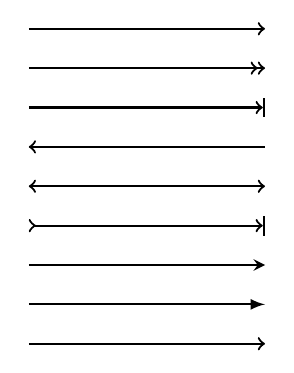
\begin{tikzpicture}[thick]
\draw[->] (0,4) -- (3,4);
\draw[->>] (0,3.5) -- (3,3.5);
\draw[->|] (0,3) -- (3,3);
\draw[<-] (0,2.5) -- (3,2.5);
\draw[<->] (0,2) -- (3,2);
\draw[>->|] (0,1.5) -- (3,1.5);
\draw[-stealth] (0,1) -- (3,1);
\draw[-latex] (0,0.5) -- (3,0.5);
\draw[-to] (0,0) -- (3,0);
\end{tikzpicture}

5.\par
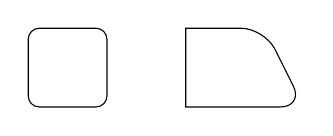
\begin{tikzpicture}
\draw[rounded corners]
(0,0) rectangle (1,1);
\draw (2,0) -- (2,1)
[rounded corners=.3cm]
-- (3,1) -- (3.5,0)
[sharp corners] -- cycle;
\end{tikzpicture}

6.\par
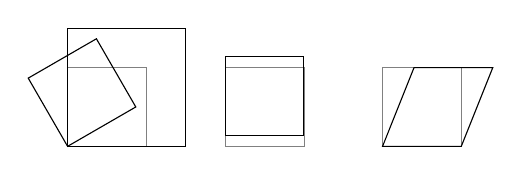
\begin{tikzpicture}
\draw[help lines](0,0) rectangle (1,1);
\draw[scale=1.5] (0,0) rectangle (1,1);
\draw[rotate=30] (0,0) rectangle (1,1);
\draw[help lines](2,0) rectangle (3,1);
\draw[yshift=4pt](2,0) rectangle (3,1);
\draw[help lines](4,0) rectangle (5,1);
\draw[xslant=0.4](4,0) rectangle (5,1);
\end{tikzpicture}

7.\par
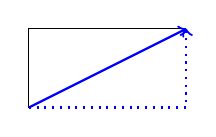
\begin{tikzpicture}
[myarrow/.style={blue,thick,->}]
\draw (0,0)--(0,1)--(2,1);
\draw[myarrow] (0,0)--(2,1);
\draw[myarrow,dotted]
(0,0)--(2,0)--(2,1);
\end{tikzpicture}

8.\par
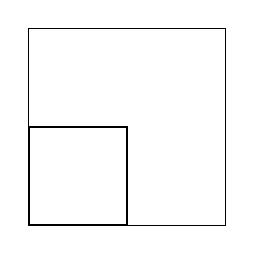
\begin{tikzpicture}
\draw (0,0) rectangle (2.5, 2.5);
\begin{scope}[thick,scale=0.5]
\draw (0,0) rectangle (2.5, 2.5);
\end{scope}
\end{tikzpicture}


\subsubsection{TikZ 文字结点}

1.\par
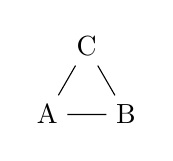
\begin{tikzpicture}
\node (A) at (0,0) {A};
\node (B) at (1,0) {B};
\node (C) at (60:1) {C};
\draw (A) -- (B) -- (C) -- (A);
\end{tikzpicture}

2.\par
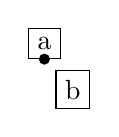
\begin{tikzpicture}
\coordinate (A) at (1,1);
\fill (A) circle[radius=2pt];
\node[draw,anchor=south] at (A) {a};
\node[draw,below right=4pt] at (A) {b};
\end{tikzpicture}

3.\par
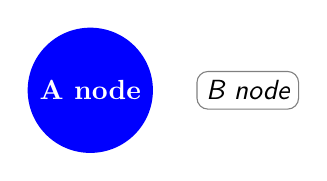
\begin{tikzpicture}
\node[circle,fill=blue,text=white,
font={\bfseries}]
(A) at (0,0) {A node};
\node[rectangle,rounded corners,
draw=gray,font={\sffamily\slshape}]
(B) at (2,0) {B node};
\end{tikzpicture}

4.\par
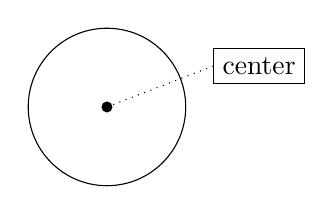
\begin{tikzpicture}
\draw (0,0) circle[radius=1];
\fill (0,0) circle[radius=2pt];
\node[draw] (P) at (15:2) {center};
\draw[dotted] (0,0) -- (P.west);
\end{tikzpicture}

5.\par
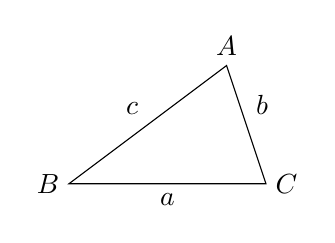
\begin{tikzpicture}
\draw (2,1.5) node[above] {$A$}
-- node[above left] {$c$}
(0,0) node[left] {$B$}
-- node[below] {$a$}
(2.5,0) node[right] {$C$}
-- node[above right] {$b$}
cycle;
\end{tikzpicture}

6.\par
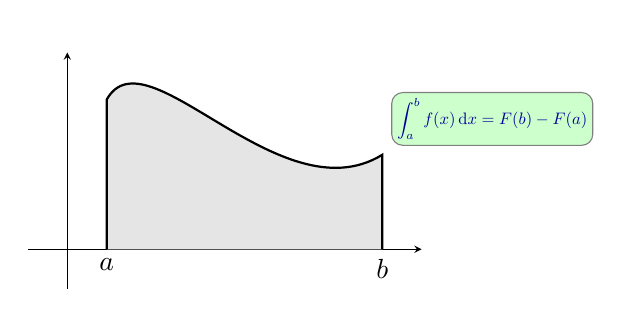
\begin{tikzpicture}
\draw[-stealth,line width=0.2pt] (-0.5,0) -- (4.5,0);
\draw[-stealth,line width=0.2pt] (0,-0.5) -- (0,2.5);
\coordinate (a) at (0.5,1.9);
\coordinate (b) at (4,1.2);
\node[below] (a0) at (a |- 0,0) {$a$};
\node[below] (b0) at (b |- 0,0) {$b$};
\filldraw[fill=gray!20,draw,thick]
(a0) -- (a) .. controls (1,2.8) and (2.7,0.4) .. (b) -- (b0) -- cycle;
\node[above right,outer sep=0.2cm, rounded corners,
fill=green!20,draw=gray,text=blue!60!black,scale=0.6]
at (b) {$\displaystyle \int_a^b {f(x)\,\mathrm{d}x} = F(b) - F(a)$};
\end{tikzpicture}

\subsubsection{在 TikZ 中使用循环}

1.\par
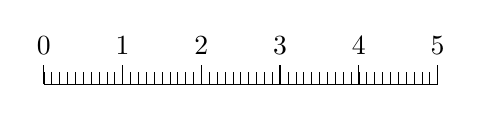
\begin{tikzpicture}
\draw (0,0)--(5,0);
\foreach \i in {0.0,0.1,...,5.0}
{\draw[very thin]
(\i,0)--(\i,0.15);}
\foreach \I in {0,1,2,3,4,5}
{\draw (\I,0)--(\I,0.25)
node[above] {\I};}
\end{tikzpicture}

2.\par
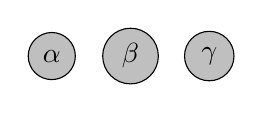
\begin{tikzpicture}
\foreach \n/\t in
{0/\alpha,1/\beta,2/\gamma}
{\node[circle,fill=lightgray,draw]
at (\n,0) {$\t$};}
\end{tikzpicture}



\section{自定义 LATEX 命令和功能}

\subsection{自定义命令和环境}

\subsubsection{定义新命令}

1.\par
\newcommand{\tnss}{The not
so Short Introduction to
\LaTeXe}
This is ``\tnss'' \ldots{}
``\tnss''

1.\par
\newcommand{\txsit}[1]
{This is the \emph{#1} Short
Introduction to \LaTeXe}
% in the document body:
\begin{itemize}
\item \txsit{not so}
\item \txsit{very}
\end{itemize}

\subsubsection{定义环境}

\newenvironment{king}
{\rule{1ex}{1ex}%
\hspace{\stretch{1}}}
{\hspace{\stretch{1}}%
\rule{1ex}{1ex}}
\begin{king}
My humble subjects \ldots
\end{king}

\subsection{编写自己的宏包和文档类}

\subsubsection{编写简单的宏包}

%This is ``\ptnss'' \ldots{}
%``\ptnss''

\subsubsection{在宏包中调用其它宏包}


\subsubsection{编写自己的文档类}


\subsection{计数器}

\subsubsection{定义和修改计数器}

\subsubsection{计数器的输出格式}


\end{document}
